%%
%% This is file `sample-sigconf.tex',
%% generated with the docstrip utility.
%%
%% The original source files were:
%%
%% samples.dtx  (with options: `all,proceedings,bibtex,sigconf')
%% 
%% IMPORTANT NOTICE:
%% 
%% For the copyright see the source file.
%% 
%% Any modified versions of this file must be renamed
%% with new filenames distinct from sample-sigconf.tex.
%% 
%% For distribution of the original source see the terms
%% for copying and modification in the file samples.dtx.
%% 
%% This generated file may be distributed as long as the
%% original source files, as listed above, are part of the
%% same distribution. (The sources need not necessarily be
%% in the same archive or directory.)
%%
%%
%% Commands for TeXCount
%TC:macro \cite [option:text,text]
%TC:macro \citep [option:text,text]
%TC:macro \citet [option:text,text]
%TC:envir table 0 1
%TC:envir table* 0 1
%TC:envir tabular [ignore] word
%TC:envir displaymath 0 word
%TC:envir math 0 word
%TC:envir comment 0 0
%%
%% The first command in your LaTeX source must be the \documentclass
%% command.
%%
%% For submission and review of your manuscript please change the
%% command to \documentclass[manuscript, screen, review]{acmart}.
%%
%% When submitting camera ready or to TAPS, please change the command
%% to \documentclass[sigconf]{acmart} or whichever template is required
%% for your publication.
%%
%%
% \documentclass[sigconf]{acmart}
\documentclass[sigplan,10pt, anonymous]{acmart}

%%
%% \BibTeX command to typeset BibTeX logo in the docs
\AtBeginDocument{%
  \providecommand\BibTeX{{%
    Bib\TeX}}}

%% Rights management information.  This information is sent to you
%% when you complete the rights form.  These commands have SAMPLE
%% values in them; it is your responsibility as an author to replace
%% the commands and values with those provided to you when you
%% complete the rights form.

\settopmatter{printacmref=false}
\setcopyright{none}
\renewcommand\footnotetextcopyrightpermission[1]{}
% \copyrightyear{2018}
% \acmYear{2018}
% \acmDOI{XXXXXXX.XXXXXXX}
% %% These commands are for a PROCEEDINGS abstract or paper.
% \acmConference[Conference acronym 'XX]{Make sure to enter the correct
%   conference title from your rights confirmation email}{June 03--05,
%   2018}{Woodstock, NY}
%%
%%  Uncomment \acmBooktitle if the title of the proceedings is different
%%  from ``Proceedings of ...''!
%%
%%\acmBooktitle{Woodstock '18: ACM Symposium on Neural Gaze Detection,
%%  June 03--05, 2018, Woodstock, NY}
% \acmISBN{978-1-4503-XXXX-X/2018/06}
\usepackage{xspace}
\usepackage{multirow}
\usepackage{subcaption}
\usepackage{booktabs}
%%
%% Submission ID.
%% Use this when submitting an article to a sponsored event. You'll
%% receive a unique submission ID from the organizers
%% of the event, and this ID should be used as the parameter to this command.
%%\acmSubmissionID{123-A56-BU3}
\newcommand{\ourmethod}{\textsc{BenchScout}\xspace}
\newcommand{\ptscpu}{PTS-CPU}
\newcommand{\ptsgpu}{PTS-GPU}
\newcommand{\id}[1]{{\itshape #1}}
\newcommand{\appname}{BenchScout}
\usepackage{xurl}
%%
%% For managing citations, it is recommended to use bibliography
%% files in BibTeX format.
%%
%% You can then either use BibTeX with the ACM-Reference-Format style,
%% or BibLaTeX with the acmnumeric or acmauthoryear sytles, that include
%% support for advanced citation of software artefact from the
%% biblatex-software package, also separately available on CTAN.
%%
%% Look at the sample-*-biblatex.tex files for templates showcasing
%% the biblatex styles.
%%

%%
%% The majority of ACM publications use numbered citations and
%% references.  The command \citestyle{authoryear} switches to the
%% "author year" style.
%%
%% If you are preparing content for an event
%% sponsored by ACM SIGGRAPH, you must use the "author year" style of
%% citations and references.
%% Uncommenting
%% the next command will enable that style.
%%\citestyle{acmauthoryear}


%%
%% end of the preamble, start of the body of the document source.
\begin{document}

%%
%% The "title" command has an optional parameter,
%% allowing the author to define a "short title" to be used in page headers.
\title[\ourmethod]{\ourmethod: Accelerating System Benchmarking with an Execution-Anchored Learning Pipeline}

%%
%% The "author" command and its associated commands are used to define
%% the authors and their affiliations.
%% Of note is the shared affiliation of the first two authors, and the
%% "authornote" and "authornotemark" commands
%% used to denote shared contribution to the research.


%%
%% By default, the full list of authors will be used in the page
%% headers. Often, this list is too long, and will overlap
%% other information printed in the page headers. This command allows
%% the author to define a more concise list
%% of authors' names for this purpose.
\renewcommand{\shortauthors}{Trovato et al.}





% \received{20 February 2007}
% \received[revised]{12 March 2009}
% \received[accepted]{5 June 2009}

%%
%% This command processes the author and affiliation and title
%% information and builds the first part of the formatted document.
\maketitle



\paragraph{Motivation.}
Benchmark suites evaluate computing platforms and system configurations by running workloads that stress subsystems such as CPU, memory, storage, process control, and accelerators.
Suites such as UnixBench and Phoronix Test Suite provide reproducible performance profiles for cloud comparison, regression testing, monitoring, and autotuning.
However, full-suite execution is costly for repeated use.
Across our testbeds, benchmark execution ranges from tens of minutes to several hours; PTS-CPU can take up to 7.5 hours, and UnixBench still requires over 25 minutes.
This overhead is hard to amortize when suites are repeatedly invoked across machines, software versions, kernel configurations, or tuning candidates.

\paragraph{Limitations of current approaches.}
Existing shortcuts are insufficient for this setting.
Static-subset methods execute a fixed set of benchmark components, but they fail to generalize across bottleneck profiles: CPU-oriented subsets may miss I/O-heavy behavior, while I/O-oriented subsets may miss compute-heavy regressions.
Execution-free predictors are cheaper, but they discard target-host execution signals and rely primarily on static host descriptors.
As a result, they are less robust to transient contention, kernel or hardware state, workload-specific behavior, and missing telemetry.
These limitations suggest that benchmark acceleration should not eliminate execution entirely; instead, it should spend a small, bounded amount of execution where it is most informative.
\begin{figure}[t]
    \centering
    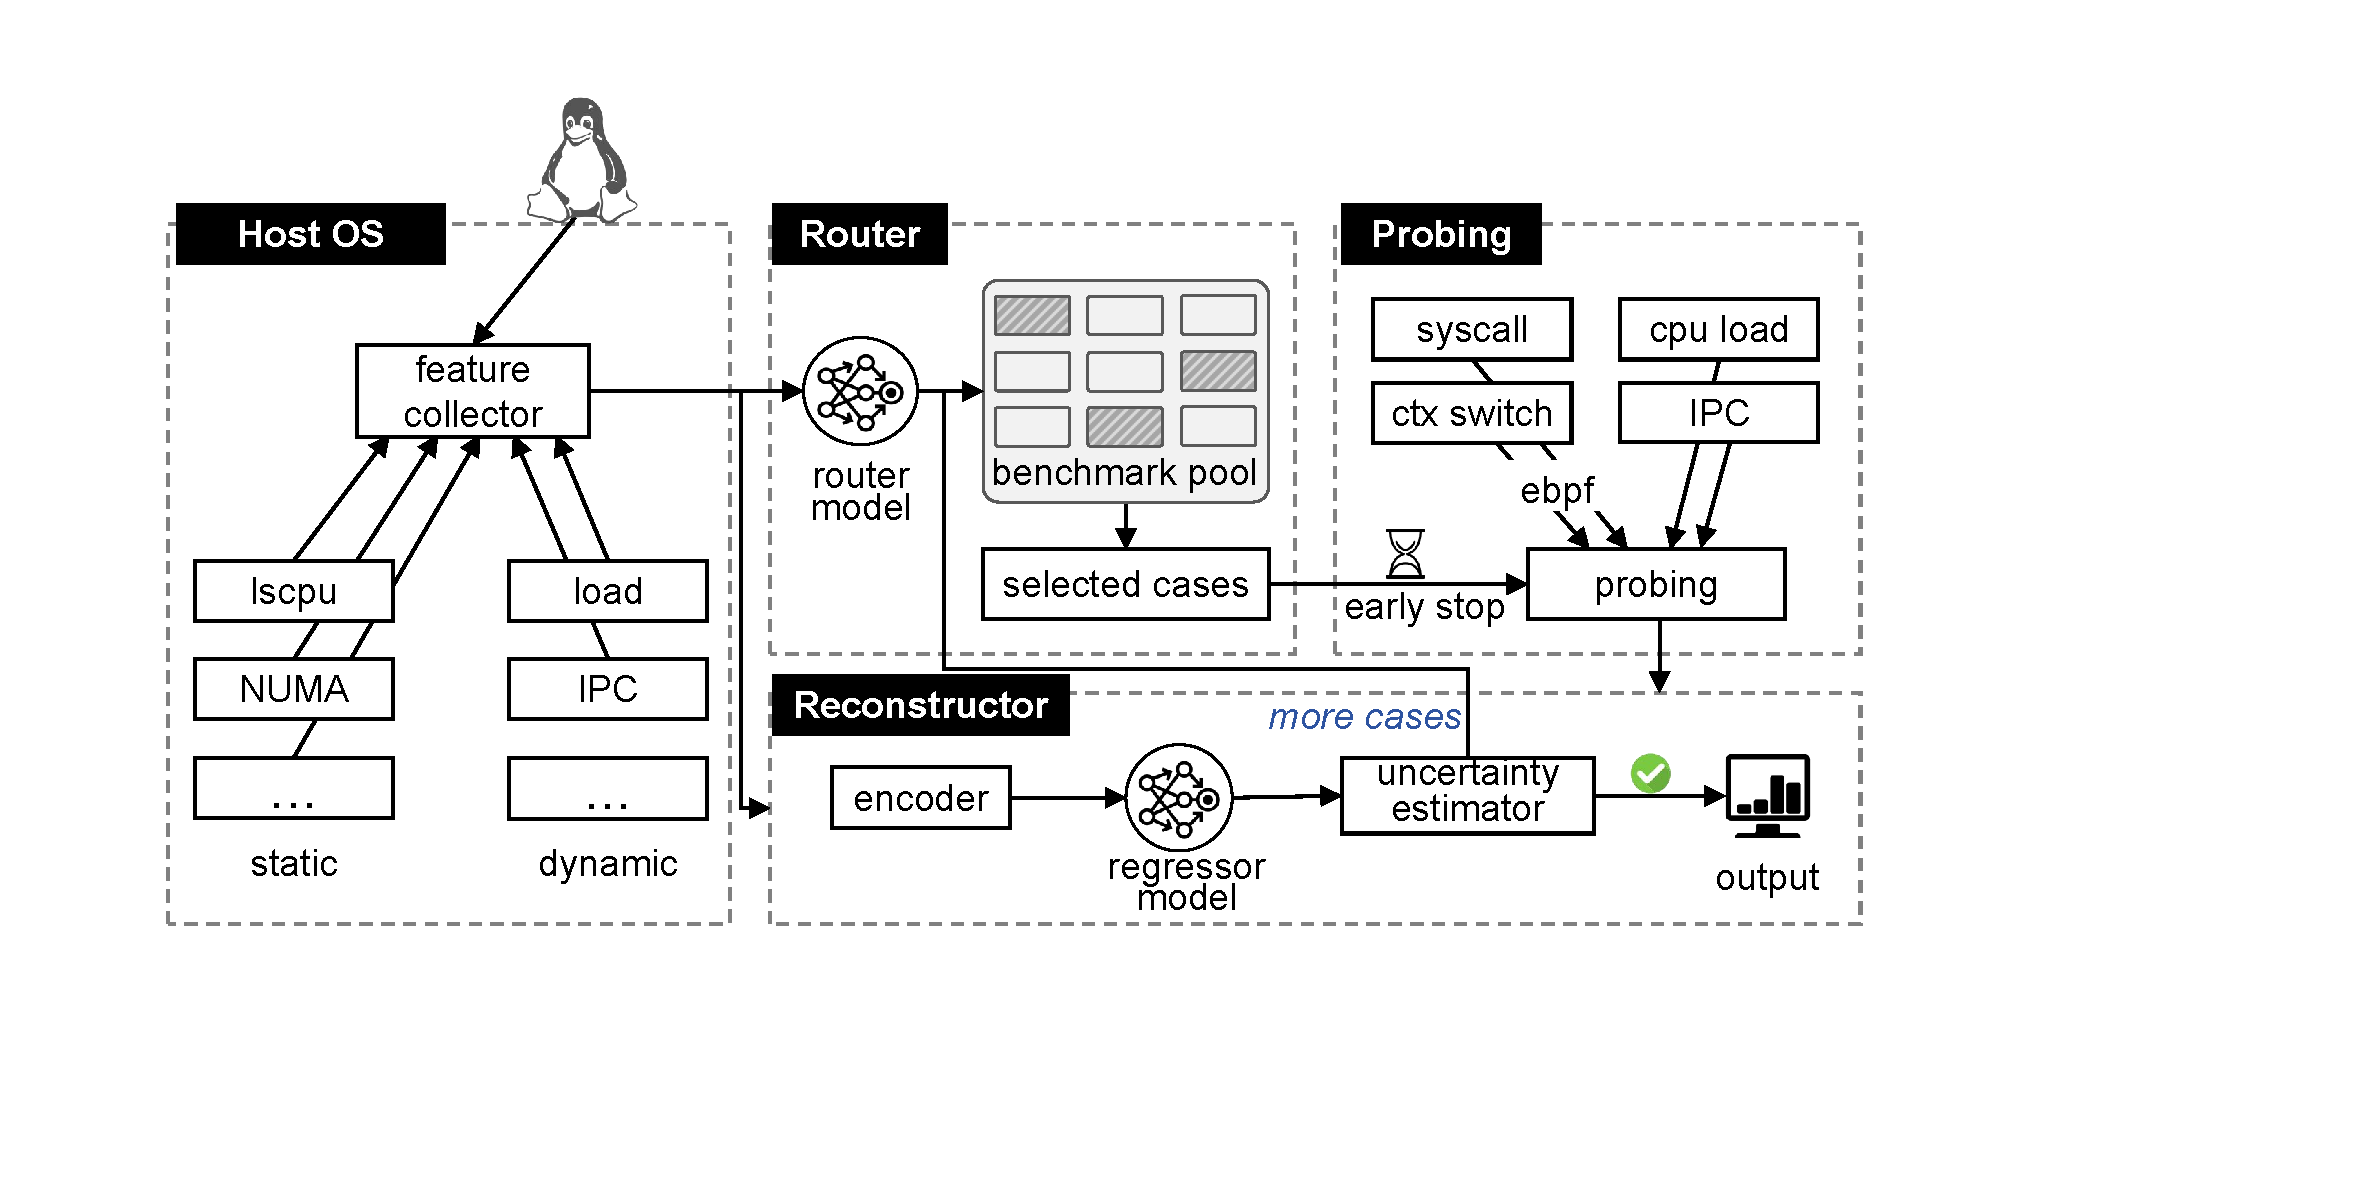
\includegraphics[width=1\linewidth]{images/mob.pdf}
    \caption{Overview of the \ourmethod architecture.}
    \label{fig:mob}
\end{figure}
\paragraph{Key ideas.}
We present \textsc{BenchScout}, an execution-anchored benchmark acceleration framework.
Its key departure from prior shortcuts is that it neither predicts benchmark results solely from static host descriptors nor commits to a fixed benchmark subset.
Instead, \textsc{BenchScout} treats a few bounded executions as informative measurements: it collects live host context, selects a small state-conditioned set of benchmark components, probes each selected component for a short fixed duration, and reconstructs the full official suite profile from the resulting sparse observations.
Because reconstruction targets the same component scores and aggregate indices reported by the original benchmark suite, \textsc{BenchScout} reduces benchmarking cost without changing the semantics of standard benchmark results.

\textsc{BenchScout} is built on three observations.
First, benchmark suites exhibit substantial subsystem redundancy: in our analysis, multiple UnixBench subtests form highly correlated clusters across five heterogeneous hosts, with CPU-oriented tests such as \textit{dhry2reg}, \textit{whetstone-double}, \textit{pipe}, and \textit{syscall} reaching correlations above 0.99.
Second, many benchmark scores can be approximated from short execution prefixes, because iterative rate tests expose stable throughput trends well before completion.
Third, production telemetry is often incomplete due to kernel, hypervisor, or isolation constraints; therefore, missing counters, blocked tracing, timeouts, and fallback paths should be encoded explicitly rather than ignored.
These observations motivate a three-stage pipeline consisting of a conditional router, a time-bounded probe estimator, and a masked sparse reconstructor.

\paragraph{System overview.}

\textbf{Conditional Router}

The router treats each benchmark component as a measurement expert. Given pre-run system context $\mathbf{x}$, it assigns each expert a relevance score and selects the Top-$K$ components. Unlike static-subset selection, this routing decision is conditioned on the current host state. Therefore, the selected components can vary across machines or runtime conditions, allowing the system to spend its limited measurement budget on the components most informative for reconstructing the full suite profile.
\begin{table*}[t]
\centering
\caption{Overall effectiveness across five heterogeneous hosts.
\ourmethod{} rows use the full pipeline: router Top-$K$, \emph{probe-model-predicted} partial scores, and reconstruction.
Wang/Tousi rows are execution-free MLP proxies~\cite{wang2019predicting,tousi2022comparative} (static hardware features only).
Execution time is in seconds; lower is better for error and time. Bold marks best among tested methods.}
\label{tab:overall-effectiveness-expanded}
\footnotesize
\setlength{\tabcolsep}{4.5pt}
\begin{tabular}{llcccccccccc}
\toprule
\multirow{2}{*}{\textbf{Suite}} & \multirow{2}{*}{\textbf{Method}} & \multicolumn{2}{c}{\textbf{M1 (32U128G)}} & \multicolumn{2}{c}{\textbf{M2 (2U8G)}} & \multicolumn{2}{c}{\textbf{M3 (4U8G)}} & \multicolumn{2}{c}{\textbf{M4 (4U16G)}} & \multicolumn{2}{c}{\textbf{M5 (8U8G)}} \\
\cmidrule(lr){3-4} \cmidrule(lr){5-6} \cmidrule(lr){7-8} \cmidrule(lr){9-10} \cmidrule(lr){11-12}
& & \textbf{Err. (\%)} & \textbf{Time (s)} & \textbf{Err. (\%)} & \textbf{Time (s)} & \textbf{Err. (\%)} & \textbf{Time (s)} & \textbf{Err. (\%)} & \textbf{Time (s)} & \textbf{Err. (\%)} & \textbf{Time (s)} \\
\midrule

\multirow{4}{*}{UnixBench} 
& Full-suite & -- & 1691.0 & -- & 1520.0 & -- & 1580.0 & -- & 1610.0 & -- & 1550.0 \\
& Wang~\cite{wang2019predicting} & 0.21 & 3.5 & 2.67 & 3.5 & 6.28 & 3.5 & 4.47 & 3.5 & 4.37 & 3.5 \\
& Tousi~\cite{tousi2022comparative} & 1.7 & 3.5 & 99.56 & 3.5 & 99.63 & 3.5 & 99.60 & 3.5 & 99.59 & 3.5 \\
& \ourmethod & $\mathbf{0.19}$ & $\mathbf{15.1}$ & $\mathbf{0.30}$ & $\mathbf{15.1}$ & $\mathbf{0.66}$ & $\mathbf{15.1}$ & $\mathbf{0.19}$ & $\mathbf{15.1}$ & $\mathbf{0.32}$ & $\mathbf{15.0}$ \\

\midrule

\multirow{4}{*}{\ptscpu} 
& Full-suite & -- & 15755.0 & -- & 12450.0 & -- & 13100.0 & -- & 13900.0 & -- & 12800.0 \\
& Wang~\cite{wang2019predicting} & 85.54 & 3.5 & 99.51 & 3.5 & 99.66 & 3.5 & 99.99 & 3.5 & 99.79 & 3.5 \\
& Tousi~\cite{tousi2022comparative} & 99.97 & 3.5 & 99.9990 & 3.5 & 99.9993 & 3.5 & 99.99997 & 3.5 & 99.9995 & 3.5 \\
& \ourmethod & $\mathbf{0.02}$ & $\mathbf{15.0}$ & $\mathbf{0.32}$ & $\mathbf{15.0}$ & $\mathbf{0.20}$ & $\mathbf{15.1}$ & $\mathbf{0.38}$ & $\mathbf{15.0}$ & $\mathbf{0.33}$ & $\mathbf{15.1}$ \\

% \midrule

% \multirow{4}{*}{\ptsgpu} 
% & Full-suite & -- & 27018.0 & -- & -- & -- & -- & -- & -- & -- & -- \\
% & Wang~\cite{wang2019predicting} & 0.26 & 3.5 & -- & -- & -- & -- & -- & -- & -- & -- \\
% & Tousi~\cite{tousi2022comparative} & 98.85 & 3.5 & -- & -- & -- & -- & -- & -- & -- & -- \\
% & \ourmethod & $\mathbf{0.18}$ & $\mathbf{15.0}$ & -- & -- & -- & -- & -- & -- & -- & -- \\

\bottomrule
\end{tabular}
\end{table*}
\textbf{Time-Bounded Probing}

For each selected component, \textsc{BenchScout} executes a fixed-duration probe rather than the complete benchmark subtest. The probe may be a lightweight micro-workload mapped to the component category, such as CPU, memory, I/O, syscall, thread, or GPU, or a timeout-bounded invocation of the original subtest. During probing, the system records prefix telemetry including elapsed wall time, resource usage, optional eBPF-derived rates, workload identity, and failure flags. A supervised probe estimator maps this telemetry to the component's official full-run score.

This stage keeps real execution in the loop, but bounds the cost of each selected component. In our default configuration, each probe lasts 4 seconds.

\textbf{Masked Sparse Reconstruction}

After probing, \textsc{BenchScout} reconstructs the complete benchmark profile from sparse observations. The reconstructor takes as input the system context, observed probe-estimated scores, binary masks indicating which components were observed, and probe durations. It outputs both component-level estimates and the aggregate suite score.

During training, historical full-run results are randomly masked to simulate partial observations. The reconstructor is then trained to recover the original full result from these masked samples. This allows it to learn correlations among benchmark components and to impute unobserved scores from sparse, probe-estimated partial information.



\paragraph{Overview of results.}
We evaluate \textsc{BenchScout} on five heterogeneous Linux hosts, ranging from small CPU-only cloud instances to a 32-vCPU server with 128~GB memory and an NVIDIA RTX 3090 Ti GPU.
UnixBench and \ptscpu{} are evaluated on all five hosts, while \ptsgpu{} is evaluated on the GPU-equipped host.
Our primary experiment measures the full end-to-end \textsc{BenchScout} pipeline: the router selects a Top-$K$ subset, the probe estimator predicts the selected components' full-run scores from bounded probe telemetry, and the reconstructor recovers the complete suite profile from these sparse probe-imputed observations.
For each host--suite pair, we apply this pipeline to all collected historical runs and report the mean suite-level relative error together with the estimated partial wall-clock time.

Table~\ref{tab:overall-effectiveness-expanded} summarizes the results.
A key point is that every partial observation fed to the reconstructor is a probe-estimator output $\hat{y}_j$, not a measured subtest score taken from the reference full run.
Thus, the reported accuracy reflects the complete router--probe--reconstruct stack under realistic probe-imputed partial observations, rather than a router-only setting that substitutes ground-truth partial scores.
Under this protocol, \textsc{BenchScout} achieves mean relative errors of $0.33\%$ on UnixBench, $0.25\%$ on \ptscpu{}, and $0.18\%$ on \ptsgpu{}.
At the same time, it reduces full-suite execution from tens of minutes or hours to approximately 15--18 seconds, corresponding to a 95--100\% reduction in wall-clock time and only 0.067--1.06\% of the original full-suite cost.

Compared with execution-free MLP baselines, \textsc{BenchScout} spends slightly more time because it keeps bounded on-host measurements in the loop, but this small execution budget substantially improves accuracy.
The execution-free baselines incur the lowest partial cost, around 3.5 seconds, but they exhibit high prediction error on \ptscpu{} and on most UnixBench hosts, with many \ptscpu{} errors approaching or exceeding 99\%.
These results show that sparse target-host measurements are essential for robust benchmark acceleration: a few bounded executions provide host-state information that static hardware descriptors alone fail to capture.




\paragraph{Conclusion}

\textsc{BenchScout} reframes benchmark-suite evaluation as conditional routing, time-bounded probing, and sparse reconstruction. Instead of replacing benchmark execution with execution-free prediction, it keeps bounded target-host measurements in the loop and uses them to reconstruct official suite profiles. Across five heterogeneous Linux hosts and multiple suites, \textsc{BenchScout} reduces wall-clock time from tens of minutes or hours to seconds while maintaining highly accurate aggregate-score estimates. By explicitly encoding missing telemetry, probe failures, and fallback paths, it remains deployable in restricted production-like environments.



\bibliographystyle{acm}
\bibliography{sample-base}


\end{document}
\endinput
%%
%% End of file `sample-sigconf.tex'.
